\chapter{The ATLAS Detector}
The primary reference for this chapter was \cite{ATLAS} and it should be consulted for further reading.
\section{Overview}
\label{atlas_overview}
The ATLAS (A Toroidal LHC Apparatus) detector \cite{ATLAS} is one of two general purpose detectors at the LHC (the other being the CMS detector). It is capable of probing both proton-proton and heavy-ion collisions.

In the coordinate system used for the ATLAS detector, the nominal interaction point is defined to be the origin; while the z-axis is defined along the beam-line, and the x-y plane transverse to the beam-line. The positive x-direction points centripetally (towards the centre of the LHC ring) and the positive y-direction is defined as pointing upwards. The azimuthal angle $\phi$ is measured around the beam axis while the polar $\theta$ angle is measured from the beam axis. Commonly used in place of the polar angle $\theta$ is pseudorapidity $\eta$, which is defined as $\eta = -\ln \tan(\theta /2)$. In cases where an object had a non-negligible mass, such as a jet, rapidity is preferred and is defined as $y = \frac{1}{2} \ln \left( \frac{E+p_{z}}{E-p_{z}} \right) $. Rapidity and pseudorapidity are favoured because (unlike the polar angle) differences in these quantities are Lorentz invariant. The azimuthal angle along with pseudorapidity is used to define a useful spacial quantity $\Delta R$, defined as $\Delta R = \sqrt{\Delta \eta ^{2} + \Delta \phi ^{2}}$. It is useful to define certain kinematic quantities in the transverse x-y plane such as transverse momentum $p_{T}$, transverse energy $E_{T}$, and missing transverse energy $E_{T}^{miss}$.

\begin{figure}
\centering
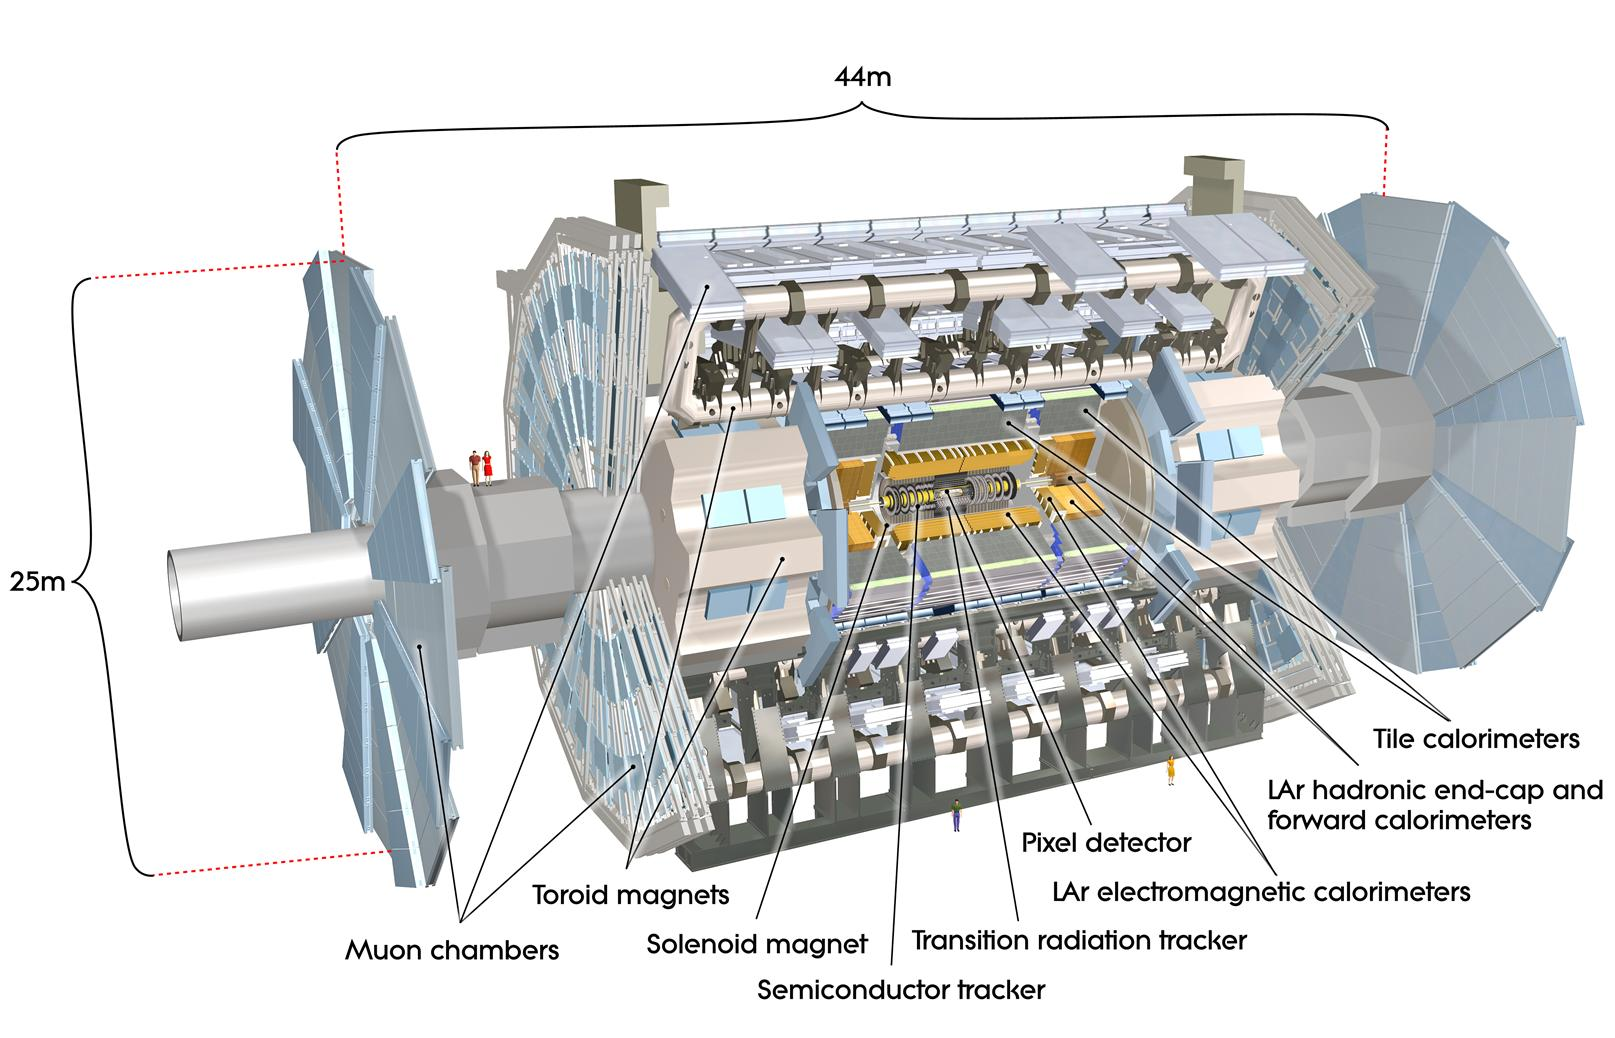
\includegraphics[scale=0.25]{images/image_AtlasDetector.png}
\caption{A cut-away view of the ATLAS detector with its dimensions and some selected components labelled. \cite{ATLAS}}
\label{AtlasDetector}
\end{figure}

The ATLAS detector itself is approximately 25 metres high, approximately 44 metres long, and weighs about 7000 tonnes. Its azimuthally symmetric design means that it is forward-backward symmetric about the interaction point (see figure \ref{AtlasDetector}). The detector's own system of magnets consist of a superconducting solenoid which surrounds the inner-detector; as well as three superconducting toroids: the barrel toroid and the two end-cap toroids. The superconducting solenoid (see figure \ref{magnet_sol}) runs parrallel with the beam-pipe and is designed to produce an axial 2 T magnetic field for the inner detector. The barrel toroid along with the two end-cap toroids (see figure \ref{magnets_tor}) serve to produce to a toroidal magnetic fields of 0.5 T and 1 T for use of the muon detectors in the barrel and end-cap regions respectively. The ATLAS detector has a 38 metre long beam-pipe section with a central chamber surrounding the interaction point. The central chamber houses the pixel detector, which forms the innermost component of the inner-detector (the other components being the SCT and TRT detectors). The inner-detector is capable of measuring the momentum of charged particles and identifying the interaction vertices, among other things. Surrounding the inner-detector is the Liquid Argon (LAr) electromagnetic calorimeter. This is a sampling calorimeter with a coverage of $|\eta | < 3.2$. This, in turn, is surrounded by the scintillating tile hadronic calorimeter (also sampling) which covers the range $ |\eta| < 1.7$. These descriptions apply to the calorimetry systems in the barrel. Supplementing the calorimetry systems in the barrel are the LAr forwards calorimeters. These extend the effect range of the calorimetry system to $ | \eta| = 4.9$ for both electromagnetic and hadronic energy measurements. The calorimetry system is surrounded by the muon spectrometer which defines the overall dimensions of the ATLAS detector.

\begin{figure}
\centering
\begin{minipage}{0.5\textwidth}
  \centering
  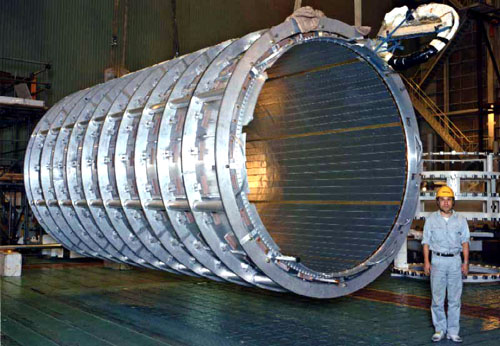
\includegraphics[width=0.7\linewidth]{images/image_solenoid_magnets.jpg}
  \captionof{figure}{The superconducting solenoid after completion of the coil winding, prior to installation. \cite{ATLAS}}
  \label{magnet_sol}
\end{minipage}%
\begin{minipage}{0.5\textwidth}
  \centering
  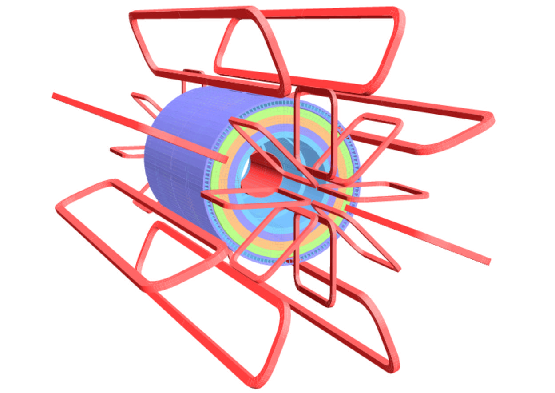
\includegraphics[width=1.0\linewidth]{images/image_toroid_magnets.png}
  \captionof{figure}{Geometry of the eight barrel toroid coils and the end-cap toroid coils. \cite{ATLAS}}
  \label{magnets_tor}
\end{minipage}
\end{figure}

The ATLAS trigger system for Run 2 is divided into two parts: the hardware-based first level trigger (L1-Trigger) \cite{l1_trigger} and the software-based high-level trigger (HLT) \cite{hlt}.

Since the design luminousity of the LHC means that high levels of radiation are present at the interaction point, the ATLAS detector needs to rely on approximately 300 tonnes of shielding in order to reduce both backgrounds and to protect the detector components and electronics from radiation damage and ageing \cite{ATLAS}. The shielding is structured in three layers, with the inner layer intended to stop high energy hadrons and secondary interactions, the second layer designed to moderate neutron radiation escaping from the first layer, and the third layer used to stop photon radiation (a by-product of the neutron capture process of the second layer).

\section{The Inner Detector}
The component of the ATLAS detector closest to the interaction point is the Inner Detector (ID) \cite{ATLAS}. It is designed to detect charged particle tracks, measure those particles' momentum, and identify both primary and secondary vertices for those charged particles above a certain $p_{T}$ threshold (nominally 0.5 GeV) in the range of $| \eta| < 2.5$. An additional function is aiding in electron identification in the range $| \eta | < 2.0$ for energies between 0.5 GeV and 150 GeV.

The ID has a cylindrical design, with has a radius of 1150 mm and a length of 3512 mm. The potential path of a charged particle passing through the three sub-detectors of the ID is illustrated in figure \ref{inner}. The ID is contained within the 2 T axial magnetic field generated by the superconducting solenoid mentioned in section \ref{atlas_overview}.
\begin{figure}
\centering
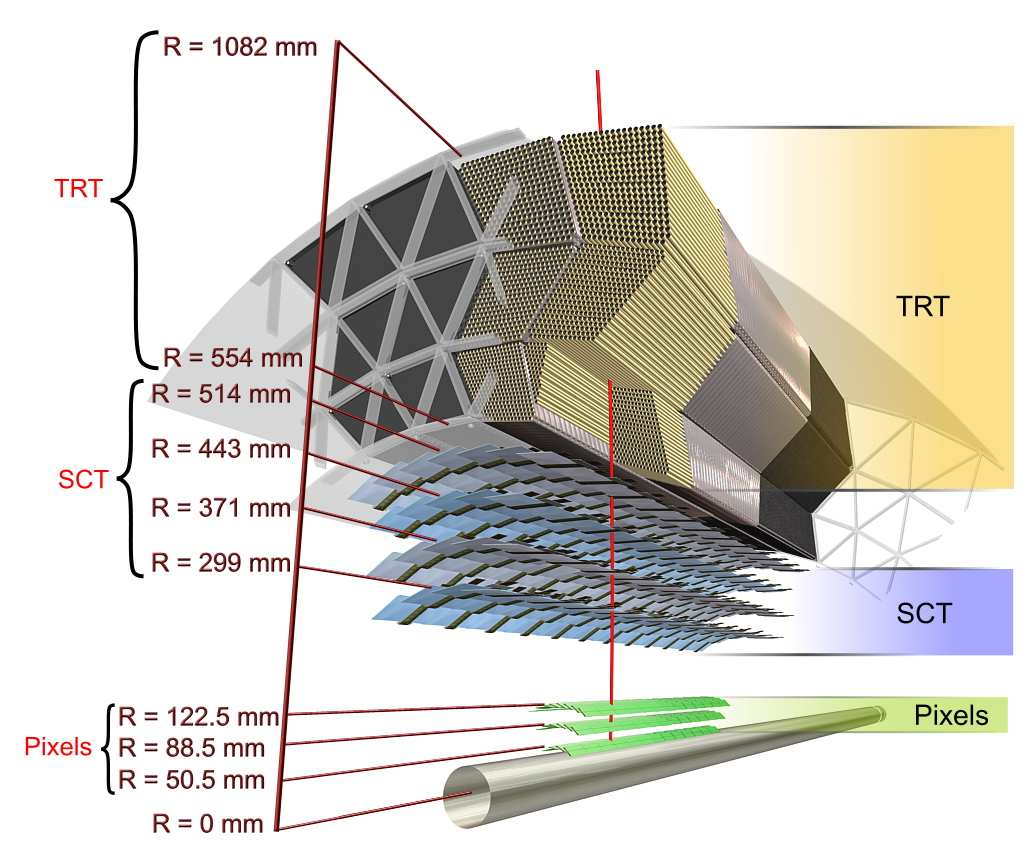
\includegraphics[scale=0.75]{images/image_inner_detector.jpg}
\caption{Illustration showing the path of a charged particle through the various layers of sub-detectors that make up the ID in the barrel region. The track passes the three cylindrical layers of the pixel layers, the four cylindrical double layers of the SCT, and finally around 36 axial straws. \cite{ATLAS}}
\label{inner}
\end{figure}
The ID is comprised of three distinct sub-detectors, with each using a different technology but all working in concert. The intrinsic resolutions of each of the sub-detectors in provided in table \ref{ID_res}. The sub-detectors with the best resoution are the precision tracking detectors: the pixel and silicon microstrip (SCT) detectors. The pixel detector is the more sensitive of the two, having 80.4 million readout channels to the SCTs' 6.3 million. It covers roughly the radial distance 50.5 mm to 150 mm from the beam-line and consists of 47 232 silicon pixels that are arranged in 1744 pixel modules. Around 90$\%$ of the pixels are $50 \mu m \times 400 \mu m$. Those remaining are slightly larger at $50 \mu m \times 600 \mu m$, these are specialised to cover the area between the chip boundaries of the pixel modules. The pixel modules themselves form three concentric barrels and two end-caps each with three discs. Usually a track coming from the interaction point will cross three pixel layers, subsequently resulting in three measurements. The pixels themselves have an adjustable threshold, any signal excess over which is considered a hit. In terms of its function, the pixel detector is essential in detecting the short-lived b-quarks and $\uptau$-leptons, and also contributes to the impact parameter measurement.
\begin{table}
	\centering{\begin{tabular}{|c|c|}
	\hline
	ID sub-detector & Intrinsic Resolution ($\mu m$) \\ \hline
	Pixel & 10($R$-$\phi$)115($z$) per sensor \\ \hline
	SCT & 17($R$-$\phi$)580($z$) per module \\ \hline
	TRT & 130 per straw \\ \hline
	\end{tabular}}
	\caption{Table listing the intrinsic resolution of each sub-detector of the ID. \cite{ATLAS}}
	\label{ID_res}
\end{table}

The SCTs cover roughly the radial distance from 299 mm to 560 mm from the beam-line. 4088 silicon-strip detector modules are formed into four concentric barrels and two end-caps, each of nine discs. They will register a hit if the pulse height exceeds a preset threshold of (usually) 1 femto Coulomb. The SCTs contribute to measurements of the momentum, impact parameter, and the corresponding vertex location from which the incident tracks originate. The SCT barrel modules are comprised of four rectangular silicon-sensor strips (two on each side), with the strips having a constant pitch of 80 $\mu m$. Two sensor at daisy chained together with a second pair being attached back-to-back with the first at a stereo angle of 40 mrad. Hence, the barrels are actually structured to be double-layered, such that a track originating from the beam-line results in eight measurements. Each of the end-cap disks is sub-divided into three rings. The modules in the middle and outer rings are formed in the same way as in the barrel, with two pairs of sensors being attached back-to-back at a stereo angle of 40 mrad. The modules of the inner ring are structured slightly differently and are made up of just two strips, attached back-to-back, at a stereo angle of 40 mrad. These two measurements per cylindrical barrel layer or disk, along with the stereo angle, are used to form discrete space-points, which are essential to the reconstruction of charged tracks in the ID (see section \ref{charged_reco}).

The Transition Radiation Tracker (TRT) covers roughly the radial distance 563 mm to 1066 mm from the beam-line. The TRT consists of 298 304 drift tubes, commonly referred to as straw-tubes, and 350 848 readout channels. The straw-tubes themselves are 4 mm in diameter and have a length of 1440 mm. The straw-tubes are filled with a gaseous mixture of Xe/CO$_{2}$/O$_{2}$ and in the centre of each straw-tube is a gold-plated tungsten wire. When a charged particle crosses the straw-tube, the gas-molecules become ionised. The central wire is positively charged and thus attracts the resulting free electrons (i.e. there is an anode wire inside a cathode tube). The subsequent charge spike on the anode constitutes a signal. This is amplified and read-out by electronics which register the fact that the straw-tube has been crossed. In terms of their geometrical layout, the straws in the barrel region form three concentric cylinders that lie parallel with the beam-axis. In the end-cap regions, the straw-tubes are orientated radially into 80 wheel resembling structures. Being the outermost of the three ID sub-detectors, the TRT deal with longer tracks and plays a significant role in measuring the momentum of those tracks.

Since it is the component of the ATLAS detector closest to the nominal interaction point, the sub-components of the ID (especially the innermost silicon pixel layers) need to be able to function even after prolonged exposure to a high-radiation environment. In fact, the cooling system of the ID must remove approximate 85 kW of heat from the ID volume at LHC design luminousity. The pixel and SCT detectors operate at a temperature of approximately -7$^{\circ}$C, while the TRT operates at room temperature.
\section{Calorimetry}
\label{calorimetry}
\subsection{Overview}
The ATLAS detector possesses a cutting-edge calorimetry system \cite{ATLAS} divided into two sub-detector systems: the Electromagnetic Calorimeter (ECal) and the Hadronic Calorimeter (HCal). Calorimeters are experimental devices used to measure an incident particle's energy. They are designed to cause the incident particle to initiate a particle shower (either electromagnetic or hadronic) and then measure the energy deposited in the calorimeter by containing the particle shower. Calorimeters are classified as either homogenous or sampling \cite{PDG}. In homogenous calorimeters, the entire volume is sensitive and contributes to the signal. In contrast, sampling calorimeters have alternating layers of absorber (dense material used to degrade the energy of the incident particle) and active medium which provides the detectable signal. Thus sampling calorimeters give an estimate of the energy of an incident particle since not all the energy is deposited in the active medium. This is in contrast to a homogenous calorimeter where the entire volume is sensitive and contributes a signal. Both the ECal and the HCal are examples of sampling calorimeters. They are both capable of energy measurements within a range of $| \eta | < 4.9$. As the names suggest, they rely on different physics interactions to function, with the ECal designed specifically for the containment of electromagnetic showers and the HCal for the containment of hadronic showers. Of the two, the ECal is the more sensitive (i.e. it has finer granularity) and is primarily concerned with measurements of electrons and photons. In contrast, the hadronic calorimeter is specialised to measure $E_{T}^{miss}$ and for jet reconstruction. It is possible for sufficiently high energy hadrons to ``punch through'' the HCal, where they can then be mistakenly reconstructed as muons in the muon spectrometer. The calorimetry system is shown in figure \ref{calorimeter}, while the granularity of each sub-detector is given in table \ref{granularity}.
\begin{figure}
\centering
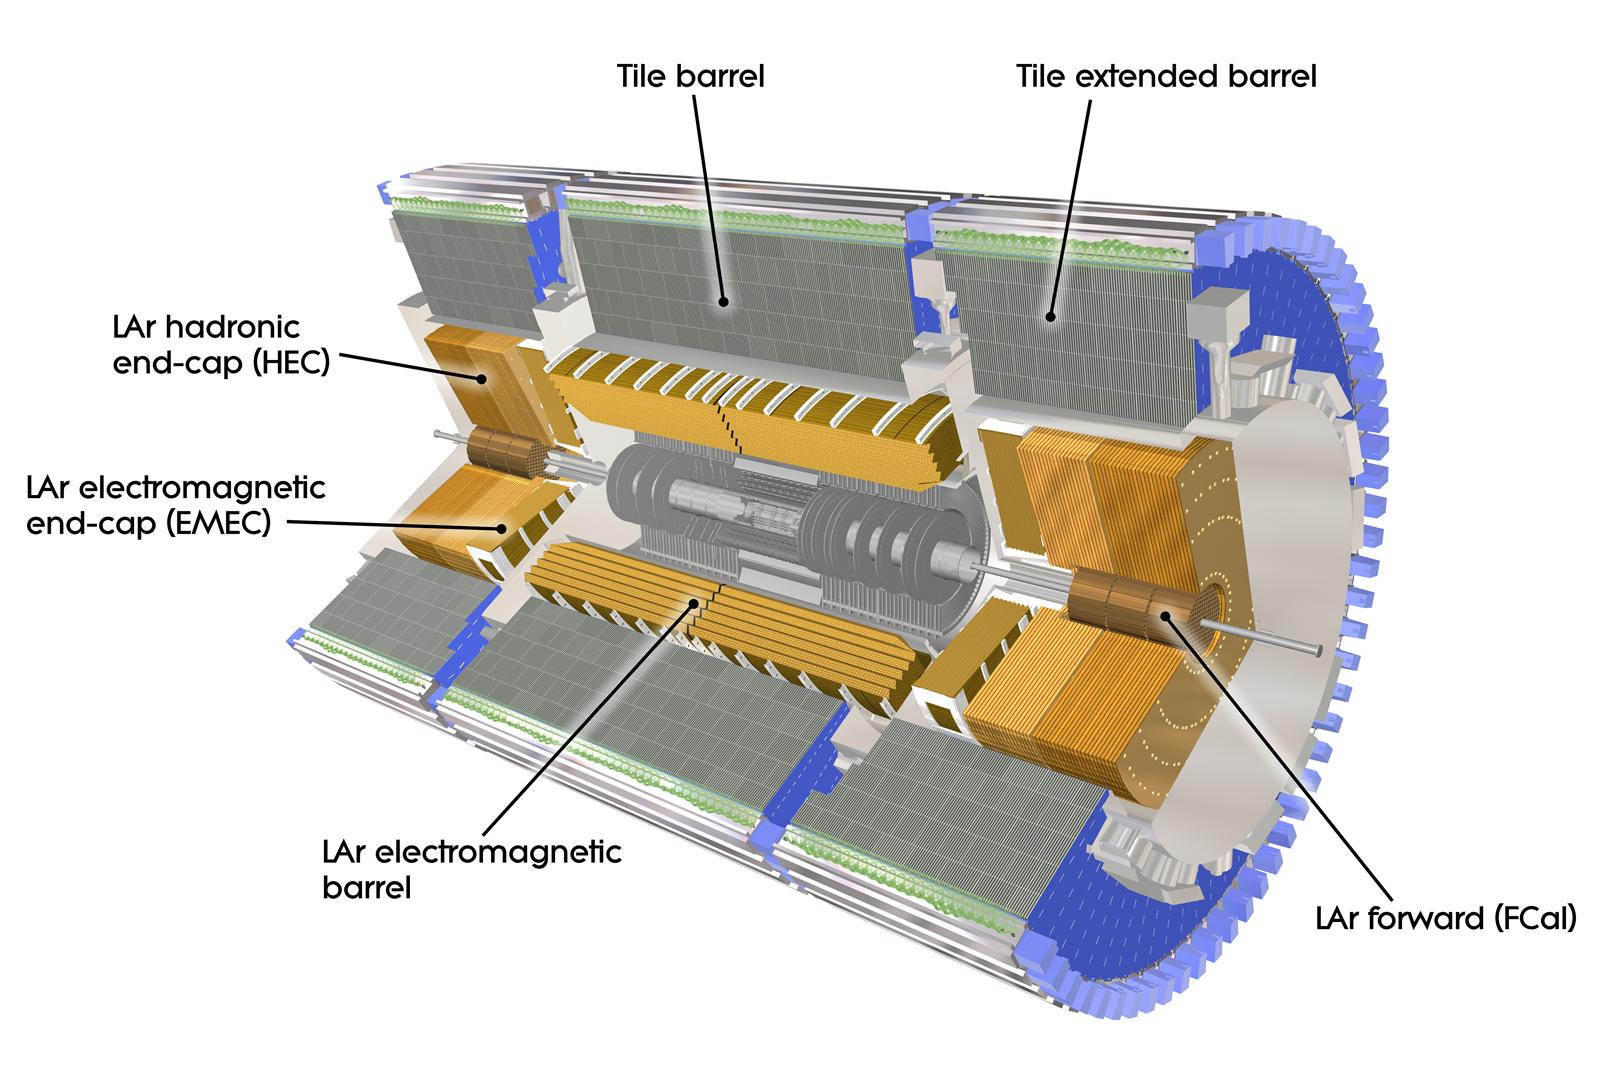
\includegraphics[scale=0.5]{images/image_calorimeter.jpg}
\caption{Illustration showing a cut-away view of the ATLAS detector's calorimetry system. \cite{ATLAS}}
\label{calorimeter}
\end{figure}
\subsection{LAr Electromagnetic Calorimeter}
The absorbers and electrodes of the ECal have an accordion geometry with full azimuthal coverage (i.e. there are no gaps, see figure \ref{accordion_design}) and pseudorapidity ranges of $| \eta | < 1.475$ for the barrel region and $1.375 < | \eta | < 3.2$ for the end-cap regions. It is divided into three layers with each layer segmented differently in $\eta$ and granularity (see table \ref{granularity}). It possesses 101760 readout channels in the barrel region, while it has 62208 in the end-cap region. The readout electrodes are located in the gaps between the absorbers and are comprised of three conductive copper layers, separated by insulating polyimide sheets. As the name suggests, the active medium is liquid argon (LAr) and, as a result, this calorimeter requires a cryostat in order to cool the system to its functioning temperature of -183$^{\circ}$C. Complementing the energy measurements provided by the ECal in the region $ | \eta | < 1.8$ is a separate thin liquid argon layer which forms the active medium for the presamplers. The presamplers serve to provide estimates of energy lost in front of the ECal. There are 7808 and 1536 readout channels in the presampler barrel and end-cap regions respectively. The active layer of LAr is 1.1 cm thick in the barrel region and 0.5 cm thick in the end-caps. Similarly to jets punching-through the HCal into the muon spectrometer, is possible for sufficiently high energy electrons or photons to pass into the hadronic calorimeter. In order to suppress this, the ECal is given a total depth of $> 33$ radiation lengths ($X_{0}$) in the barrel region and $> 24$ $X_{0}$ in the end-cap region. 

\begin{table}
	\resizebox{\textwidth}{!}{\centering{\begin{tabular}{|c|cc|cc|}
	\hline
	\textbf{Cal. Layer} & \multicolumn{2}{c|}{\textbf{Barrel}} & \multicolumn{2}{c|}{\textbf{End-Cap}}  \\ \hline
	 & Granularity ($\Delta \eta \times \Delta \phi$) & Coverage & Granularity ($\Delta \eta \times \Delta \phi$) & Coverage  \\ \hline
	 \multicolumn{5}{|c|}{\textbf{LAr Electromagnetic Calorimeter}} \\ \hline
	Presampler & $0.025 \times 0.1$ & $ | \eta | < 1.52$ & $0.025 \times 0.1$ & $1.5 < |\eta| < 1.8$  \\ \hline
	1st layer & $0.025/8 \times 0.1$ & $|\eta| < 1.40$ & $0.050 \times 0.1$ & $1.375 < | \eta | < 1.425$ \\
	 & $0.025 \times 0.025$ & $1.40 < | \eta | < 1.475$ & $0.025 \times 0.1$ & $1.425 < | \eta | < 1.5$ \\
	 & & & $0.025/8 \times 0.1$ & $1.5 < | \eta | < 1.8$ \\
	 & & & $0.025/6 \times 0.1$ & $1.8 < | \eta | < 2.0$ \\
	 & & & $0.025/4 \times 0.1$ & $2.0 < | \eta | < 2.4$ \\
	 & & & $0.025 \times 0.1$ & $2.4 < | \eta | <2.5$ \\
	 & & & $0.1 \times 0.1$ & $2.5 < | \eta | < 3.2$ \\ \hline
	 2nd layer & $0.025 \times 0.025$ & $| \eta | < 1.40$ & $0.050 \times 0.025$ & $1.375 < | \eta | < 1.425$ \\ 
	 & $0.075 \times 0.025$ & $1.40 < | \eta | < 1.475$ & $0.025 \times 0.025$ & $1.425 < | \eta | < 2.5$ \\
	 & & & $0.1 \times 0.1$ & $2.5 < | \eta | < 3.2$ \\ \hline
	 3rd layer & $0.050 \times 0.025$ & $| \eta | < 1.35$ & $0.050 \times 0.025$ & $1.5 < | \eta | < 2.5$ \\ \hline
	 \multicolumn{5}{|c|}{\textbf{Tile Calorimeter}} \\ \hline
	 All except last layer & $0.1 \times 0.1$ & & $0.1 \times 0.1$ & \\ \hline
	 Last layer & $0.2 \times 0.1$ & & $0.2 \times 0.1$ & \\ \hline
	 \multicolumn{5}{|c|}{\textbf{LAr Hadronic End-Cap Calorimeter}} \\ \hline
	 & & & $0.1 \times 0.1$ & $1.5 < | \eta | < 2.5$ \\ 
	 & & & $0.2 \times 0.2$ & $2.5 < | \eta | < 3.2$ \\ \hline
	 \multicolumn{5}{|c|}{\textbf{LAr Forward Calorimeter}} \\ \hline
	 & & & Granularity $\Delta x \times \Delta y$ (cm) & Coverage \\ \hline
	 1st module & & & $3.0 \times 2.6$ & $3.15 < | \eta | < 4.30$ \\
	 & & & $(3.0 \times 2.6)/4$ & $3.10 < | \eta | < 3.15$ \\
	 & & & & $4.30 < | \eta | < 4.83$ \\ \hline
	 2nd module & & & $3.3 \times 4.2$ & $3.24 < | \eta | < 4.50$ \\
	 & & & $(3.3 \times 4.2)/4$ & $3.20 < | \eta | < 3.24$, \\
	 & & & & $4.50 < | \eta | < 4.81$ \\ \hline
	 3rd module & & & $5.4 \times 4.7$ & $3.32 < | \eta | < 4.60$ \\
	 & & & $(5.4 \times 4.7)/4$ & $3.29 < | \eta | < 3.32$, \\
	 & & & & $4.60 < | \eta | < 4.75$ \\
	\hline
	\end{tabular}}}
	\caption{Table listing the granularity of each the sub-detectors of the calorimetry system. \cite{ATLAS}}
	\label{granularity}
\end{table}

\begin{figure}
\centering
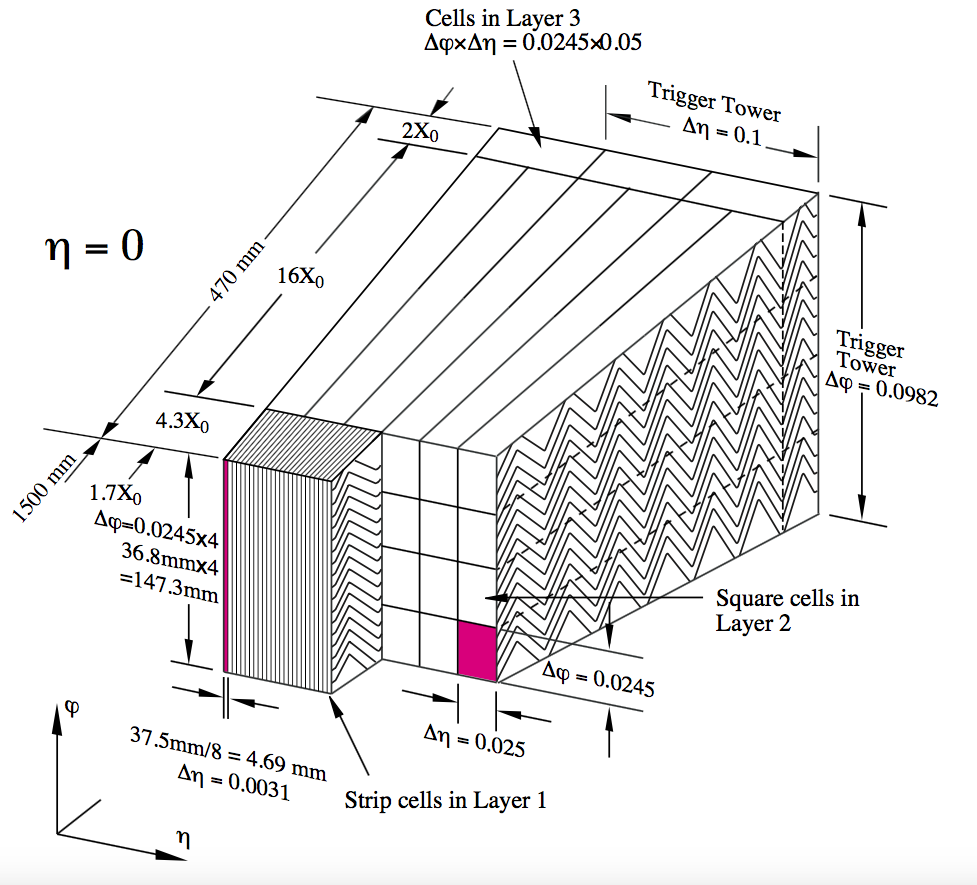
\includegraphics[scale=0.4]{images/accordion_design.png}
\caption{Illustration of an ECal barrel module showing its full azimuthal design. $X_{0}$ is the radiation length. \cite{ATLAS}}
\label{accordion_design}
\end{figure}
\subsection{Hadronic Calorimeters}
\subsubsection{Tile Calorimeter}
Enveloping the ECal is the Tile Calorimeter. It consists of three distinct structures: the barrel region, which covers the range $ | \eta | < 1.0$, and the two extended barrel regions which cover the range $ 0.8 < | \eta | < 1.7 $. As the name suggests, scintillating tiles form the active medium while steel is used as the absorber. The Tile Calorimeter occupies the annular volume defined by inner and outer radii of 2.28 m and 4.25 m respectively. It is radially segmented into three layers, while it is azimuthally segmented into 64 modules with a total of 5760 and 4092 readout channels in the barrel and end-cap regions respectively.
\subsubsection{LAr Hadronic End-Cap Calorimeter}
Located directly behind the end-cap ECal (and in fact sharing the same LAr cryostat), the LAr Hadronic End-cap Calorimeter (HEC) is comprised of two separate wheels. The HEC has a range of $ 1.5 < | \eta | < 3.2$ and does have some overlap with the Forward Calorimeter. Copper plates are used as the absorber, with the plates being interleaved with LAr which serves as the active medium. It has a total of 5632 readout channels.
\subsubsection{LAr Forward Calorimeter}
Integrated into the end-cap cryostat, the LAr forward calorimeter is divided into three modules (in each of the end-caps) with a total of 3524 readout channels. It provides hadronic calorimetry measurements in the extreme forward region, $3.1<|\eta|<4.9$. The first module consists of copper and is designed to primarily measure energy deposited through electromagnetic interactions. The other two consist of tungsten and are optimised for the measurement of energy deposited through strong interactions (hadronic showers). LAr is again used as the active medium.
\section{Muon Spectrometer}
The outermost sub-detector of the ATLAS detector is the Muon Spectrometer \cite{ATLAS}. It is designed to take muon measurements through the deflection of their tracks due to the magnetic field provided by its large superconducting air-core toroid magnets. It has approximately 1 million readout channels and occupies the annular volume defined by the inner and outer radii of 4.25 m (close to the calorimeter) and 11 m (the full radius of the ATLAS detector) respectively. The magnetic deflection is primarily due to the barrel toroid in the range defined by $ | \eta | < 1.4$, and primarily due to two smaller end-cap magnets inserted into each end of the barrel toroid for the range $1.6 < | \eta | < 2.7$. There is also a region $1.4 < | \eta | < 1.6$ where magnetic deflection is due to both, hence this is called the transition region. The Muon Spectrometer also possesses a separate trigger and high-precision tracking chambers. In the barrel region, these chambers are arranged in three cylindrical layers (parallel to the beam-axis) with radii 5m, 7.5 m, and 10 m from the beam-axis. The chambers in the transition and end-cap regions form wheel structures at $z \approx 7.4$ m, $10.8$ m, $14$ m, and $21.5$ m that lie orthogonal to the beam-axis.

There are four types of chambers found in the muon spectrometer. The Monitored Drift Tubes (MDTs) and Cathode Strip Chambers (CSCs) together form the precision-tracking chambers. They provide precise measurements of the track coordinate in the direction defined by the magnetic field. The MDTs cover the broad range $|\eta | < 2.7$. The CSCs provide additional tracking measurements for the forward region $2 < | \eta | < 2.7$ and are specially designed with higher granularity than the MDTs in order to cope with the high background rate in the forward region.

The other two chamber types: the Resistive Plate Chambers (RPCs) and Thin-Gap Chambers (TGCs) are used as part of the muon spectrometer's specialised muon trigger. The RPCs are used in the barrel, while the TGCs are used in the end-caps. These chambers cover the range $ | \eta | < 2.4$. The trigger chambers also play a role in measuring the muons' coordinates in the direction perpendicular to that measured by the precision-tracking chambers, as well as identifying the bunch-crossings from their resultant tracks.

\section{Forward Detectors}
The ATLAS forward region is covered by three small detectors \cite {ATLAS}. The first two, LUCID (LUminousity measurement using Cherenkov Integrating Detector) and ALFA (Absolute Luminousity For ATLAS), are located approximately 17 m and 240 m from the interaction point respectively. They are designed to measure the luminousity delivered to ATLAS. The third system ZDC (Zero-Degree Calorimeter) has an essential part in determining the centrality of heavy-ion collisions and is located approximately 140 m from the interaction point.
\section{Trigger System}
\label{trigger_system}
The ATLAS trigger system \cite {ATLAS} was briefly mentioned in section \ref{atlas_overview}. This section expands on that but is still only a brief overview. The ATLAS trigger system is divided into two distinct levels, namely, the hardware-based Level-1 (L1) Trigger \cite{l1_trigger} and the software-based High-Level Trigger (HLT) \cite{hlt}. The HLT refines the selections made by its predecessor and, when necessary, applies additional selection criteria. The L1 trigger uses only a small amount of the potentially available detector information in order to make a decision as to whether or not the event should be ignored or examined further. It makes this decision in a mean time of 2.5 $\mu$s per event, reducing the event rate from the 30 MHz proton-proton bunch crossing rate to 100 kHz. The L1 trigger makes this decision using important information from a sub-set of the sub-detectors. It searches for the high $p_{T}$ leptons, photons, and jets; as well as high missing transverse energy $E_{T}^{miss}$ or high total transverse energy $E_{T}^{tot}$. Calorimeter information is based off reduced granularity measurements in order to save time on the decision as to whether to keep the event. It also identifies Regions-of-interest (RoI) and passes this information onto the HLT. Using full granularity and precision, the HLT examines the RoI's with a mean event processing time of 200 ms, further reducing the event rate to 1 kHz. 